\chapter{Detailed Design and Implementation}
\label{ch:implementation}

\section{Introduction}
\label{sec:implementation-introduction}
This project contains 5 different components that are deployed in different \
places:
\begin{enumerate}
    \item the robot application (deployed and running on the actual robot)
    \item A Web server that handles TLS termination
    \item the proxy server that acts as an intermediary between the user \
            controlling the robot and the robot; \
            it runs in a google cloud virtual machine
    \item an angular web client that is used to control the robot; \
            it is \
            deployed in the same cloud as the proxy server, but runs in the \
            user's browser
    \item the cloud processor that reconstructs images sent by the robot, \
            optionally detects/tracks people and then forwards them to the \
            proxy server; for performance reasons, it runs on the same \
            virtual machine as the proxy server
\end{enumerate}

Each component's detailed design and implementation will be detailed below.
A deployment diagram detailing the interactions between componetns can be found \
in figure ~\ref{fig:deployment-diagram}

\begin{figure}[ht]
    \label{fig:deployment-diagram}
    \centering
    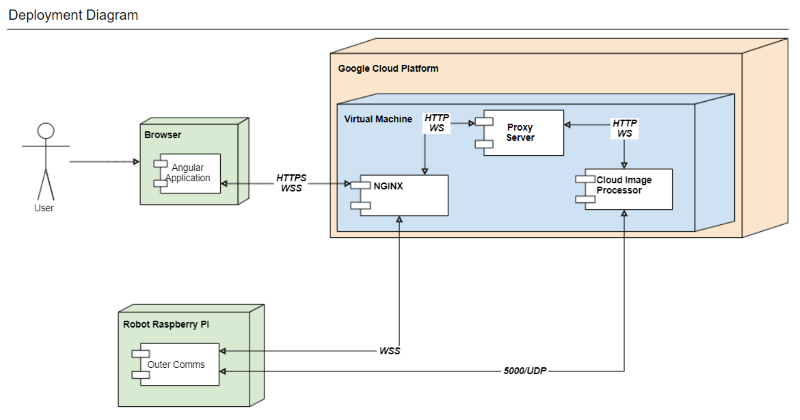
\includegraphics[keepaspectratio]{img/deployment4.PNG}
    \caption{Deployment Diagram}
\end{figure}

\section{Robot Application}
\label{sec:robot-application}
I have chosen to run the robot application on a Raspberry PI 3 both \
because of the support for high-level development languages (Python, \
JavaScript, as opposed to VHDL/Verilog), and because of the support for \
third party modules/application (in this instance, RabbitMQ).

\subsection{Hardware}
\label{subsec:implementation-robot-hardware}

Physically, the robot consists of 2 modular platforms, 4 wheels with associated \
DC engines, a Raspberry PI, a motor shield for the raspberry, batteries and a \
camera, all connected with wires.
The 2 modular platforms were joined with screws to form the chassis of the \
robot.
The 4 engines were attached to the chassis at both ends using screws, and the \
rubber wheels were mounted on the engines.
The Raspberry PI microcomputer was attached to one of the platforms forming the \
chassis using screws.
As for the motor shield, it came separately from the shield connector, so \
I had to glue it to the shield connector with solder.
Attaching the shield connector to the raspberry was simple, all I had to do was match \
the pins.
The motor shield has separate controls for 4 engines, along with pins for \
current and ground.
For this project, I used the current for motors to power the raspberry as well, \
though for a production setup the raspberry should be powered by a different \
set of batteries.
The camera was attached to the raspberry using a flex cable connector.
In order to reduce costs, I decided to use my phone as a 4G/LTE connector, however \
there are modules to connect the Raspberry PI to 4G/ LTE (not GPRS, which is \
considerably slower).
The phone was connected to the raspberry using USB 2.
In order to meet the recommended power requirements for the motors I needed \
6 AA batteries.

\begin{figure}[ht]
    \label{fig:robot1}
    \centering
    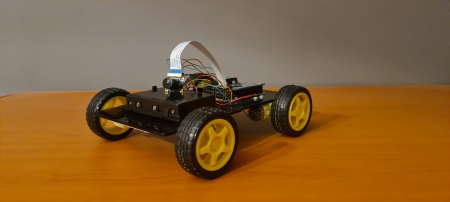
\includegraphics[keepaspectratio]{img/robot1d.jpg}
    \caption{Robot 1}
\end{figure}

\begin{figure}[ht]
    \label{fig:robot2}
    %\centering
    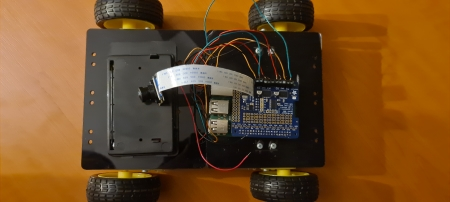
\includegraphics[keepaspectratio]{img/robot2d.jpg}
    \caption{Robot 2}
\end{figure}

\begin{figure}[ht]
    \label{fig:robot3}
    %\centering
    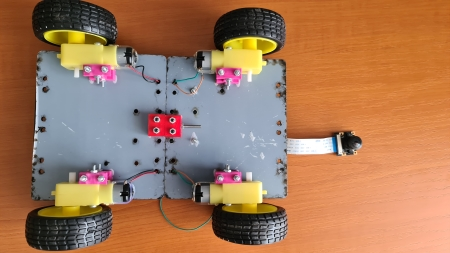
\includegraphics[keepaspectratio]{img/robot3d.jpg}
    \caption{Robot 3}
\end{figure}


\subsection{Software}
\label{subsec:implementation-robot-software}

From a software point of view, it consists of 2 independent modules communicating \
with one another via RabbitMQ queues.
The modules are engine control and external comms.
The engine control module is implemented in python and controls the 4 wheels \
independently and can make the robot go forward, reverse and steer.
The motors themselves are controlled using the pip module \
\textbf{adafruit\-circuitpython\-motorkit}, which is written by the company \
that produced the motor shield.
Using the module, each motors is assigned a positive throttle to move forward \
and a negative throttle to go in reverse.
However, after assembling the robot, I noticed that I mounted some motors in \
reverse.
In order to fix this issue, when assigning a throttle to a motor, I multiply \
that throttle by an int representing the forward direction (1 or -1, \
depending on the direction the motor was mounted).
\begin{verbatim}
class Motor:

    def __init__(self, adafruit_motor: DCMotor, forward=1):
        self.motor = adafruit_motor
        self.forward_direction = forward
        self.throttle = 0

    def move(self, throttle):
        self.motor.throttle = throttle * self.forward_direction
\end{verbatim}

Using domain-driven design, I discovered that possible classes are Motor (DC Motor \
controlling a wheel) and Engine, that controls all motors.
The Motor class is an adapter for the Afadruit DCMotor class, and contains \
the forward direction (1/-1) and a method to set speed.
The Engine class has the four motors as properties and public methods to \
fo forward, backward and steer.
Since the motor location is important, each motor has its own instance variable.
The class also contains a list with all motors, useful for setting the same \
throttle to all motors.
When going straight forward, backward or stopping, the same throttle is set on \
all motors.
The left/right direction is controlled by a float variable that can take values \
between 1 and -1.
Positive values represent a right direction (with 1 being max \
right), while negative values represent a left direction (with -1 \
being max left).
When steering left, the motors on the left side are set a throttle smaller \
than the one on the right side by a factor that depends on how much the \
user wants the robot to steer.
The mechanism for steering right is similar, except the motors on the right side \
are assigned a smaller throttle.
\begin{verbatim}
def steer(self, direction):
    print('Steer', direction)
    """
    :param direction:
        -1 -> left
        1 -> right
    :return:
    """
    if direction == 0:
        self.forward(self.throttle)
    elif direction < 0:
        self._steer_left(direction * -1)
    else:
        self._steer_right(direction)

def _steer_right(self, intensity):
    intensity = 1 - intensity
    self.bottom_right_motor.move(self.throttle * (1 - intensity))
    self.top_right_motor.move(self.throttle * intensity)

def _steer_left(self, intensity):
    intensity = 1 - intensity
    self.top_left_motor.move(self.throttle * intensity)
    self.bottom_left_motor.move(self.throttle * intensity)

\end{verbatim}
As mentioned in the analysis phase, the engine control component listens on \
a queue, a RabbitMQ queue, more precisely, for commands.

\begin{figure}[ht]
    \label{fig:engine-class-uml}
    %\centering
    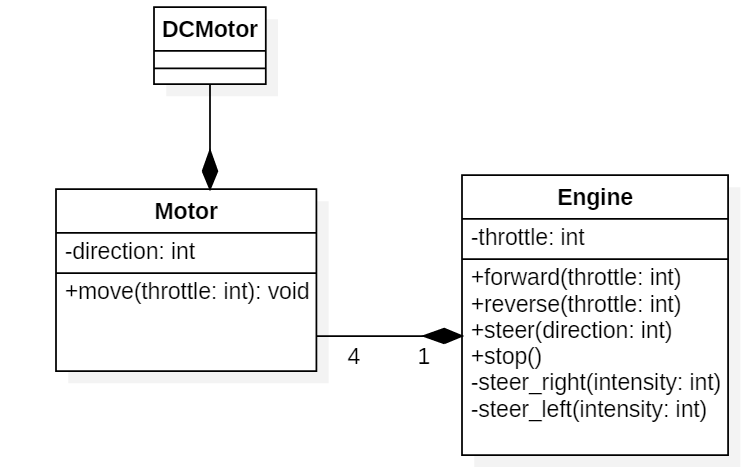
\includegraphics[width=15cm, height=30cm,keepaspectratio]{img/engine-class-uml.png}
    \caption{Engine Control Class UML}
\end{figure}


The external comms has 2 roles: capture video from camera to transmit it to the \
server, and listen for commands from the remote server in order to transmit them \
to the engine control via RabbitMQ.
I decided to have image transmission and commands listener in a single component \
because they are logically related (they represent the interaction with the outside \
world) and both depend on active internet connection.
Once can easily notice that this component is event-based, reacting to either \
external events (commands transmitted via websockets) or internal events (\
a timer for transmitting new images).
In Python, this would require 2 threads/processes, one for image transmission \
and one for the command listener.
However, since JavaScript is an event-driven language, it is better suited for \
the tasks and can do both of them in a single thread.
Still, the outer comms component was not written in plain JavaScript.
It was written in TypeScript, which is a superset of JavaScript that \
is more type-safe than plain JavaScript.
Unlike JavaScript, TypeScript cannot be run directly, it must first be compiled \
into JavaScript, which can then be run in the NodeJS runtime.
The outer comms expects the commands to be json objects containing the direction \
and the throttle for the engines.


When developing the robot components, I connected the raspberry to my home \
wireless router, and thus I was able to ssh into the raspberry, upload files \
and start and monitor the components.
However, after I connected the raspberry to the phone's 4G/LTE network, I \
could no longer ssh into the robot, and had to find a new way to monitor \
components and upload files.
The solution I found was to assign the robot a DNS for dynamic IP from noip.com .
This allowed me to open specific ports from the robot to the internet (mainly \
22 for SSH and 15672 for RabbitMQ UI), so that I could access them from another \
network (my home network).
Even though the performance was far from ideal (for free tier), it was enough \
in order to start/stop processes on the robot, view logs and inspect/publish rabbit \
messages.

The robot is also the first component involved in determining the FPS rate, the \
other component being the cloud image processor.
The robot sets a timer at which it captures a new image and sends it to \
the image processor.

\section{UDP Packing-Unpacking algorithm}
\label{sec:udp-packing-algorithm}

\subsection{Overview}
\label{subsec:udp-pack-overview}

The UDP Packing\-Unpacking algorithm plays an important roles in the \
system, since it handles the image transmission from the robot \
to the cloud.
The algorithm turns a buffer of variable size (the image to be \
transmitted) into multiple small \
buffers that are UDP-safe (from the size perspective), and can then \
reconstruct the initial buffer.

In order for a buffer to be sent successfully over UDP, it \
cannot exceed a certain limit, which most people agree is \
around 500 bytes.
Thus, I had to split the original buffer into multiple small \
buffer.
However, since the UDP protocol doesn't guarantee the order of arrival \
(or even the arrival for that matter), each packet must have \
2 unique identifiers: an identifier for the buffer to \
which it belongs (global identifier), and an identifier for \
its place in the buffer (local identifier).
I decided that a good option for the global identifier \
would be the timestamp at which the image was taken, \
expressed in milliseconds.
As for the local identifier, I chose it to be an \
increasing index for each packet.
Additionally, in order to reconstruct the original buffer, \
we would have to know the total number of packets from \
that buffer.
However, it only needs to be sent once, not with every \
packet, so I decided it should be sent only with the \
first packet (named head buffer).
To sum up, the original buffer is split into several \
mini\-buffers (packets) of about 400 bytes size, and each \
packet has a header with its creation timestamp, \
its order index and, in the case of the packets with \
order index 0, the total number of packets.

When receiving packets and reconstructing the image, \
I also had to take into account that the packets will \
probably come out of order.
In order to easily group packets belonging to the same \
original buffer, I created a Map in which the keys are \
the buffer's timestamp, and the values are objects \
that contain the total number of packets in the \
original buffer (which can be determined once packet \
0 arrives), and a list of the packets generated from \
that buffer.
Once all the packets from a buffer arrive, they are \
ordered according to their local index, and the \
original buffer can be reconstructed.

\subsection{Algorithm}
\label{subsec:udp-packer-algorithm}
I have described the packing and the unpacking algorithms in the \
pseudo-code samples below, which are similar to python.

\begin{verbatim}
    // Image deconstruction algorithm psesudo-code
    // jpeg is the buffer to be decomposed
    timestamp = int(time.time() * 1000)
    udpPackets = []
    initialDataSize = PACKET_MAX_SIZE - HEADER_PACKET_HEADER_SIZE
    dataBuffer = jpeg[0:initialDataSize]
    udpPackets.push(new HeaderPacket(dataBuffer, timestamp, len(jpeg))
    page = 1
    dataPacketSize = PACKET_MAX_SIZE - DATA_PACKET_HEADER_SIZE
    jpegOffset = initialDataSize

    while True:
        end = min(jpegOffset + dataPacketSize, len(jpeg))
        currentBuffer = jpeg[jpegOffset:end]
        udpPackets.push(new DataPacket(currentBuffer, timestamp, page))
        page++

        if end == len(jpeg):
            break
        else:
            jpegOffset = end
\end{verbatim}

\begin{verbatim}
    // Image reconstruction algorithm
    packetMap = new HashMap()
    while True:
        packet = readPacket()
        timestmap = packet.readTimestamp()
        if timestmap not in packetMap:
            packetList = new PacketList()
            packetMap.put(timestmap, packetList)
        else:
            packetList = packetMap.get(timestamp)

        packetList.packets.push(packet)
        if not packetList.imageDescriptor and packet.isHeaderPacket():
            packetList.imageDescriptor = packet.getImageDescriptor()

        if packetList.imageDescriptor and len(packetList.packets) == packetList.imageDescritptor.noOfPages:
            sort(packetList.packets, by=lambda x: x.readPage())
            imageData = [x.getData() for x in packetList.packets].join(b'')
            delete udpMap[timestamp]
            emit(imageData, timestamp)
\end{verbatim}

\subsection{Implementation}
\label{subsec:udp-packer-implementation}
As for the actual implementation, I had to write the same algorithm \
twice.
Since the robot's outer comms component would be in charge of sending \
images, the first implementation would have to be in NodeJS.
Technically, I only needed to implement the packing part of the \
algorithm, which generates the udp packets from the image buffer.
However, in order to validate that the algorithm works, I had to \
implement the unpacking as well in order to make sure the udp packets \
are valid and that the original image can be reconstructed.
Then I had to re-implement the unpacking in python so that the \
image processor can read the udp packages and reconstruct the \
original image as well.
Since by this time I had already finished the NodeJS algorithm, I \
no longer had to re-implement the packing in python, since I could \
use the packets generated in NodeJS.

The actual UML class diagrams for the NodeJS implementations can be found \
in figure ~\ref{fig:udp-packer-class-uml}.
Unlike other languages like Java (where interfaces are used to specify common \
behavior for polymorphism) or Python (which doesn't even have interfaces), \
in TypeScript, interfaces can be used both for polymorphism and for describing \
data types in JSON format, with all properties being public.
Another difference from Java is the \textbf{?} operator used for the property \
\textit{imageDescriptor} in the interface \textit{UdpPacketList}.
This is used to mark the property as optional, since when first constructing the \
\textit{UdpPacketList} when the first packet from the image arrives, we don't \
know if that is the header packet, which is the only one who can generate an \
image descriptor.

As convention, private properties and methods are marked with a \textbf{\-}, \
while public properties and methods are marked with a \textbg{\+}.
Static methods are underlined.

In the \textit{UdpPacket} class, the \textit{buffer} property is a binary buffer \
that contains both headers and actual data.
The first two static methods, \textbf{headerPacket} and \textbf{dataPacket}, act \
as constructors because TypeScript doesn't allow multiple constructors for a class.
Another option would have been to make the \textit{UdpClass} abstract and create \
another two classes that would extend the base class: \textit{HeaderUdpPacket} \
and \textit{DataUdpPacket}.
However, the two types of packets were too similar and had very few differences, \\
so I decided to go with different constructors.
The method \textit{getImageDescriptor} throws an error if the packet is not a \
header packet.
The class constructor is private and only accepts the full buffer that \
contains both the data and the headers.
Since the class\' only private property is the full buffer, all getters from \
it need to read binary data from the buffer and then decode it.

In the \textit{UdpPacker} class, the property \textit{udpMap} is a Javascript \
Map object (similar to Java HashMap), which is faster than the commonly-used \
object for retrieving key-value data.
The \textit{imageEmitter} property is an instance of the NodeJS-specific \
\textit{EventEmitter} class (since this is NodeJS-specific, it won't work \
by default in the browser, though some frontend frameworks have their \
own custom implementation of EventEmitter).
The \textit{EventEmitter} class is part of the NodeJS implementation of the \
Observer Pattern, which allows other micro-tasks to wait for an event and its \
associated data (the observable object decides what data is associated to each \
event) from the observable micro-task to occur.
However, the observers do not execute immediately, but only when the active \
micro-task finishes executing.
This allows multiple micro-tasks to wait for a specific event.
The static \textit{pack()} method packs a buffer into multiple udp packets.
The \textit{addPacket()} method adds a packet to the udpMap and, when it \
discovers that all the packets from an image have been received, emits an event \
with that image and its timestamp on the imageEmitter.

The Python implementation is somewhat similar to the NodeJS one, with a few \
exceptions generated by the difference in technologies.
First of all, \textit{ImageDescriptor}, \textit{PacketDescriptor} and \
\textit{UdpPacketList} are classes, since Python doesn't support interfaces.
The \textit{UdpPacket} class is almost identical to the NodeJS implementation.
As for the \textit{UdpPacker} class, it has been renamed in Python into \
\textit{UdpUnpacker} (since packing wasn't implemented).
The \textit{udpMap} property is now a Python dict, while the \
\textit{imageEmitter} property doesn't exist (since Python doesn't have \
JavaScript's asynchronous code execution).
The \textit{pack()} method doesn't exist, while the \textit{addPacket} method \
returns a tuple which can contain the image buffer and timestamp, if the \
added packet is the last packet to arrive from an image, or an empty buffer \
and 0 for timestamp.


\begin{figure}[ht]
    \label{fig:udp-packer-class-uml}
    %\centering
    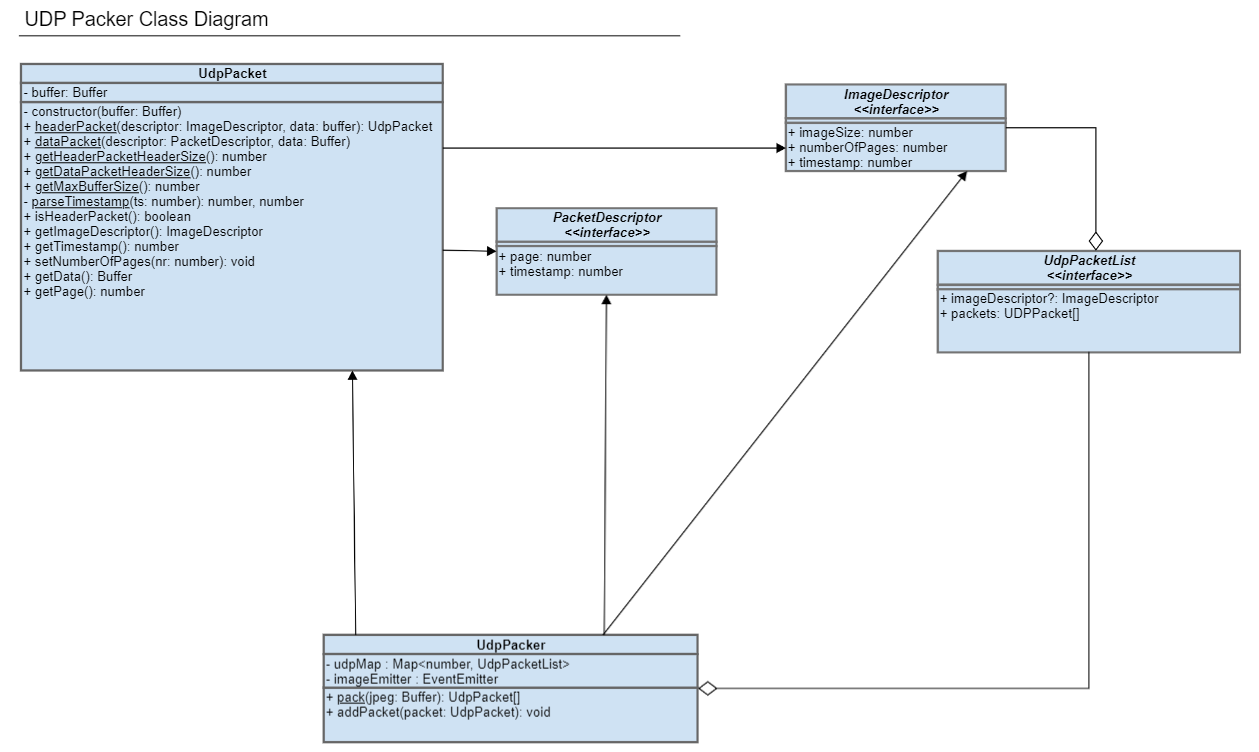
\includegraphics[width=15cm, height=30cm,keepaspectratio]{img/udp-packer-uml-class.png}
    \caption{Udp Packer-Unpacker UML Class Diagram}
\end{figure}

\subsection{Encoding}
\label{subsec:udp-packer-encoding}
In order to minimize the number of created udp packets, the headers must take \
as few bytes as possible, which means they must be instances of the smallest \
integers possible without breaking functionality.
However, neither Python nor Javascript have multiple classes of ints based on \
the number of bytes usable.
Javascript has only one class, \textit{number} that is used to represent both \
integers and floats.
Internally, it is stored as a 64-bit float represented in format IEEE-754, with \
52 bits reserved for mantissa, 11 for exponent and 1 for sign.
Additionally, JavaScript also support \textit{BigInts} which do not have an \
upper limit.
Python, on the other hand, has only one type for integers: \textit{int}.
Internally, each int is represented using C structures, not the C types for \
integers, meaning Python doesn't have an upper or lower limit for integers.
However, both languages contain APIs to write ints of different types and \
sizes to buffers.

In NodeJS, the \textit{Buffer} class has methods to write ints of different \
types and sizes to a buffer (for instance, \textit{Buffer.prototype.writeUInt32LE}, \
which takes as arguments the number to be written and the offset at which to \
write it).
In Python, the \textit{struct} module is used.
The \textit{struct.unpack} is used to read data types from a binary buffer.
It takes as arguments a string in which the types of data are specified, \
as shown in figures ~\ref{fig:udp-packer-python-structs} and \
~\ref{fig:udp-packer-python-endiannes}.
Following this format, 4-byte integers can be read as following: \
\begin{verbatim}
unsigned_short = struct.unpack('<H', buffer[0:2])[0]
\end{verbatim}

\begin{figure}[ht]
    \label{fig:udp-packer-python-structs}
    %\centering
    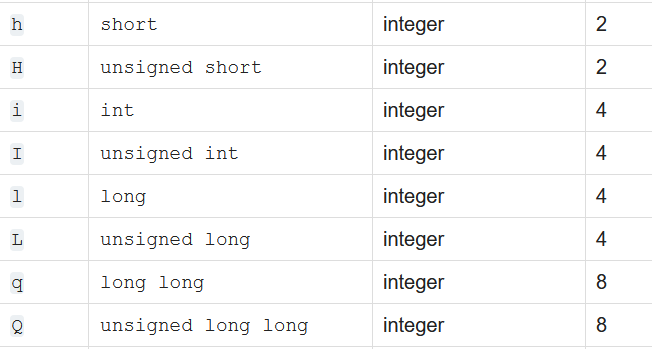
\includegraphics[keepaspectratio]{img/python-structs.png}
    \caption{Python Struct Encodings\footnote{https://docs.python.org/3/library/struct.html}}
\end{figure}

\begin{figure}[ht]
    \label{fig:udp-packer-python-endiannes}
    %\centering
    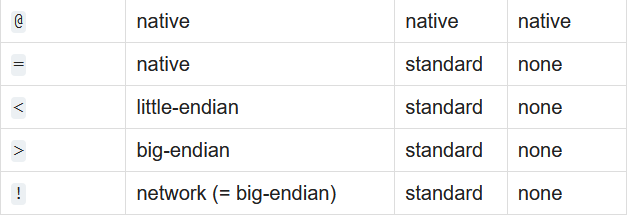
\includegraphics[keepaspectratio]{img/python-endiannes.png}
    \caption{Python Struct Endiannes\footnote{https://docs.python.org/3/library/struct.html}}
\end{figure}

Having decided how to write the headers, I needed to decide on the actual \
size in which the header's number would be written.
I decided that all header numbers would be transmitted as integers to maximize \
the numbers that can be written.
The first header information was the image size.
During tests I noticed that most images being transmitted had around 60kb, with \
only a few reaching 63 KB.
I decided that 2 bytes weren't enough to transmit this information (the maximum \
unsigned number that can be represented on 2 bytes is $2^{16} - 1 = 65535$, which \
is pretty close to 64512, the size of a 63 KB image), as it wouldn't allow \
increases in image size.
So I decided that image size should be represented on 4 bytes.
The number of pages was the next variable.
Considering an image of 60 KB, this can be split into 154 packets, well below \
the maximum unsigned number that can be represented on 1 byte (255), which would \
be used for images sizing 99 KB.
So I decided to represent the number of pages using an unsigned 1-byte number.
The timestamp, however, represented an issue.
The current timestamp is $1\_592\_655\_360$, which cannot be represented on \
4 bytes, but it could easily be represented on 6-bytes.
However, there is no integer type that can be represented on 6-bytes, only on 4 \
bytes and 8 bytes.
In order to save an additional two bytes per packet, I decided to split the \
timestamp into seconds ($1\_592\_655$) and milliseconds ($360$).
The seconds can be easily represented on 4 bytes, while the seconds can be \
stored on 2 bytes.
The final structure of the data packets can be found below, in figure \
~\ref{fig:udp-packer-packet-composition}.

\begin{figure}[ht]
    \label{fig:udp-packer-packet-composition}
    %\centering
    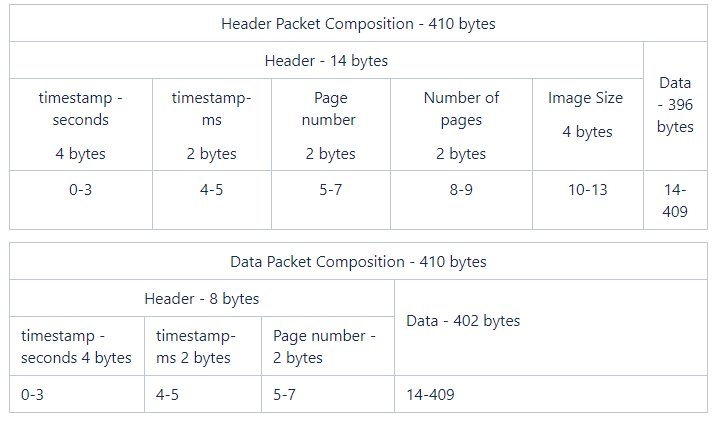
\includegraphics{img/packet-composition.PNG}
    \caption{Packet Composition}
\end{figure}


\section{Web Server}
\label{sec:web-server}
Both the proxy server and the web client sit behind a reverse proxy.
The reverse proxy's job is to handle TLS termination, and thus ensure that \
the system is immune to man\-in\-the\-middle\-attacks.
This is done primarily for the websocket server, since no information is \
passed to the http server.
The reverse proxy is also in charge of serving the web client files (html, \
js, css), which are available on the \textit{/static/} location.
The reverse proxy uses a self\-signed certificate.

When it came to choosing a reverse proxy to deploy, I had two choices: \
Apache and nginx.
Although there are web servers exist, these two are the most popular \
on the internet right now.
According to \
\footnote{https://www.hostingadvice.com/how\-to/nginx\-vs\-apache/} \
and \footnote{https://www.tecmint.com/why\-nginx\-better\-than\-apache/}, \
nginx is better suited among other things for serving static content and \
for serving as a reverse proxy to an application server.
These are the two use cases that I need a web server for, so I decided to \
go with nginx.



\section{Proxy Server}
\label{sec:implementation-proxy-server}
The Proxy Server is the central component that intermediates the communication \
between the robot and the controller.
Similar to the robot outer comms component, it consists mainly \
of reactions to events.
These events are either http requests or websockets events.
And just like the outer comms, the best language to develop the proxy server \
is NodeJS.
Since this component only redirects messages to other clients, it contains \
no classes, just server declarations and message handling, probably being \
the simplest component.
However, this is the component that ties all the other components together.

The Proxy Server runs in a virtual machine on Google Cloud.
It requires the following ports to be open:
\begin{itemize}
    \item \textbf{TCP 22} used by the ssh server. Login is done using public-private keys
    \item \textbf{TCP 443} used by the HTTPS and Websockets server
    \item \textbf{UDP 5000} used by the cloud processor. More details on this in \
            ~\ref{sec:implementation-cloud-processor}
\end{itemize}
The proxy itself created embedded HTTP and Websockets server on \
which it actively listens, but these are not open to the exterior.
The web server listens on port 443, terminates TLS connections and \
then routes the un-encrypted traffic to the HTTP and Websockets servers.

The proxy allows all users who are aware of its existence to view the video \
feed.
However, it protects the commands and the video generator with two distinct keys.
This way, it ensures that no one (not even a controller) can directly impersonate \
the robot and transmit its own video feed.
Having the controllers login before being able to issue commands ensures \
that bystanders or other malicious people cannot hack the drone.

The way the proxy server works is the following: (see figure ~\ref{fig:proxy-activity-diagram}):
\begin{itemize}
    \item After proxy startup, it waits for new websocket connections
    \item Once a new connection has been initialized, that connection can \
            begin receiving video feed
    \item Each connection can attempt to authenticate with a secret token
        \begin{itemize}
            \item If the secret token belongs to the controller, the proxy server \
                    begins accepting drone control events from that connection
            \item If the secret token belongs to the cloud processor, the proxy \
                    server begins accepting image events from that connection
            \item If the secret token belongs to neither cloud processor nor controller, \
                    it is invalid and the websocket connection is terminated
        \end{itemize}
    \item Authenticated connections are still valid to receive video feed
    \item The proxy continues transmitting vide ofeed and redirecting commands until it \
            receives a SIGINT signal and exits
\end{itemize}

\begin{figure}[ht]
    \label{fig:proxy-activity-diagram}
    %\centering
    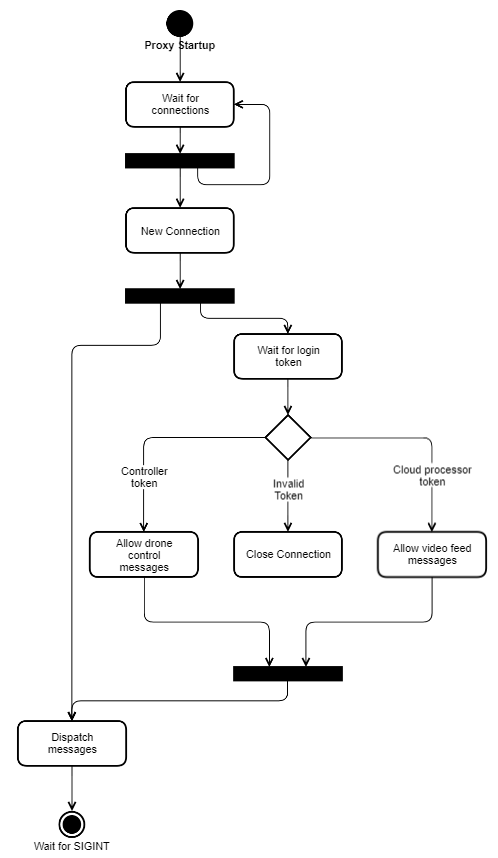
\includegraphics[width=10cm, height=20cm,keepaspectratio]{img/proxy-activity.PNG}
    \caption{Proxy Server Activity Diagram}
\end{figure}

Whenever the proxy server receives an image event from the cloud processor, it \
forwards that event to the connected clients.
During implementation, I had to choose between 2 methods of delivering images \
to the clients.
The first method was to push images through websockets to the clients, which is \
the method that was implemented in the end.
The other method was to use multipart http response.
In the multipart implementation, an http route is configured to send multiple \
images to the caller (browser) up until the caller closes the connection.
If a html image element had such a route as src, then the image would \
update itself each time the server sent another image.
Although the multipart implementation would considerably simplify the frontend \
application (there would probably be no more need for websockets), I found that \
it was more rigid than the websockets implementation.
While websockets allows for random data to be passed to clients (like image, \
time spent in processing, time the image was taken), the multipart implementation only allows \
the image itself to be transmitted, without any other metadata.
As this would have made it impossible to calculate the time by the image \
in each phase of its existence (image creation, transport to cloud \
processor, processing, transport to client), I decided to go with the \
websocket-based transport.

The proxy server was designed to run in NodeJS.
Just like the outer comms component, it was written in TypeScript, which \
was then compiled to JavaScript, which in turn could be run in NodeJS.

The proxy server also contains an embedded HTTP server.
This server has no active functionality, it is only required to setup \
websockets on the server.

Initially, both the proxy server and the cloud processor were designed to \
run inside docker containers running on a Kubernetes cluster.
However, after some initial tests, I decided against the idea.
In order to run the 2 services as docker containers, I first had to \
create a Kubernetes cluster consisting of at least 2 virtual machines.
Once the cluster was created, several Kubernetes system pods were \
automatically deployed on it.
I decided it was more cost-effective to run both components on the same \
virtual machine than running a Kubernetes cluster formed of 2 virtual \
machines that also ran Kubernetes system pods besides my own pods.
Still, I decided to leave the Dockerfiles, since they showed how each \
component should be configured.



\section{Web Client}
\label{sec:implementation-web-client}
The Web Client allows users to see the live video feed and issue commands.
It is an Angular 9 application that uses Typescript and compiles to html, \
css and javascript files optimized for browsers.
The application consists of 2 separate angular components: image-viewer and \
control.

Since both the image viewer and the control components rely on a websocket \
connection to receive image, respectively transmit commands, I decided to \
create an Angular singleton service which will handle all websocket communication.
This service was named \textbf{CloudSocketService} (the suffix \
\textit{Service} is added by default by Angular to all services).
This service was then injected into both components.

As for deployment, as I mentioned above, the Angular application is compiled \
into several html, css and javascript files.
I deployed these files on the same virtual machine on which the proxy server \
and the cloud processor.
They are served by the nginx web server mentioned above.


\section{Cloud Image Processor}
\label{sec:implementation-cloud-processor}
The cloud processor is the most complex component in the project.
The overall logic can be seen in diagram ~\ref{fig:cloud-processor-activity-diagram}.

\begin{figure}[ht]
    \label{fig:cloud-processor-activity-diagram}
    %\centering
    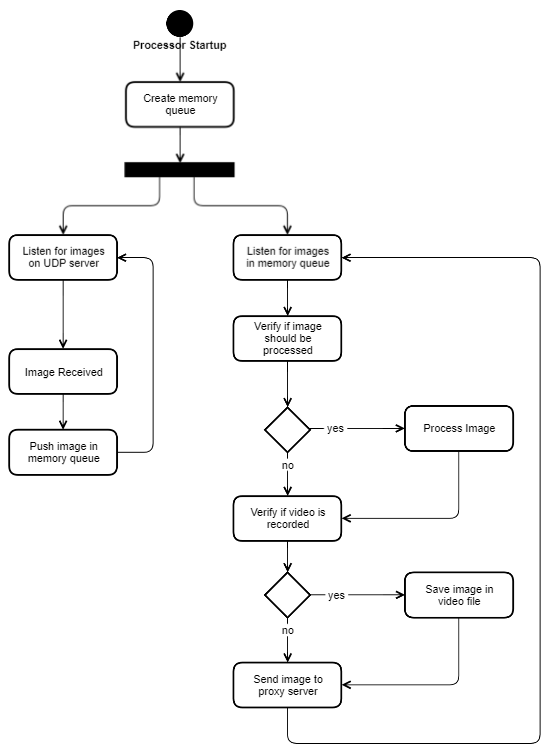
\includegraphics[keepaspectratio]{img/cloud-processor-activity.PNG}
    \caption{Cloud Processor Activity Diagram}
\end{figure}

As can be easily from the diagram, the cloud processor is composed of \
two different mini-components: one component that listens for images \
sent by the drone on a udp server, and one mini-component that \
processes each image and forwards it to the proxy server.
I considered splitting the cloud processor into 2 distinct components, \
but in the end I decided to have the two mini-components form a single \
component for the following reasons:
\begin{enumerate}
    \item \textbf{Resource use} If the 2 mini components were \
            separate components, I would probably have needed a dedicated \
            queue server (possibly rabbitmq); this server would have been \
            deployed on the same virtual machine on which the two components \
            would have run (thus increasing load on the machine), or in a \
            separate virtual machine, thus increasing costs.
    \item \textbf{Increased performance} Since the 2 mini-components are \
            connected, they can share a memory queue;
            this eliminates the overhead brought by network communication, \
            increasing the processing speed for each image, and thus \
            increasing throughput
\end{enumerate}

Since the two mini-components are connected, they should be \
implemented in the same language.
While the udp listener can be implemented in any language, the image \
processor should be implemented in Python because of the very large \
number of python libraries dedicated to image processing.

The image processing mini-component is expected to run in parallel to the \
component that parses the images.
This way, while one component receives and processes udp frames, the \
other component processes an already received image, increasing \
throughput and FPS.
Ideally, they would run in different threads, allowing them to share \
memory.
However, because of the Python GIL Lock
\footnote{https://wiki.python.org/moin/GlobalInterpreterLock}, only one \
thread in a process can execute at a time.
This allows for concurrent, but not parallel execution of threads.

As a result, the two mini-components will have to be run in different \
processes, communicating with each other through a multiprocessing \
queue.

\subsection{UDP Listener}
\label{subsec:implementation-udp-listener}
The UDP listener is more lightweight than image processor, so this will \
be the component that will be started in a different process (the \
\textit{UDPServer} class will extend the Python \
\textit{multiprocessing.Process} class) and will receive in constructor \
the multiprocessing queue in which it will write unpacked images.
Min-component memory footprint is important because Python doesn't \
implement the copy-on-write mechanism that is implemented by other \
languages when it comes to creating new processes.
Instead, Python pickles (serializes) all affected data and sends it \
to the new process.

The UDP Listener is the second component involved in \
deciding the FPS rate, after the robot software.
The UDP listener, after having rebuilt an image, empties the \
memory queue it shares with the processor.
This is because the time it takes the processor to process an \
image might be considerably higher than the time it takes \
the udp listener to reconstruct image, thus making it \
possible for images to accumulate in the queue.
Since we are interested in live video feed, older images \
are less important than new images, and as such they \
can easily be deleted.
Because some images might be randomly deleted, the final \
FPS rate can be lower than the FPS rate set by the robot, \
without any way to determine how much it can differ.

\subsection{Image Processor}
\label{subsec:implementation-image-processor}
This mini-component is more heavy-weight than the udp listener \
because it deals with the tensorflow and tensorflow-gpu libraries, \
the latter of which cannot be pickled so that it can be sent to a \
subprocess.

In the processing phase, an object detection learning configured to \
detect people is applied on the image.
As mentioned in ~\ref{subsec:analysis-object-detection}, I decided to \
use a MobileNet neural network thanks to its combination of speed \
and relative precision.
The specific network that I used was trained on images with size \
300x300, so it is for this resolution that it will offer the best \
performance.
After having run some performance tests, I discovered that the neural \
network offers similar performance to images sized 600x600 to images \
sized 300x300.
For this reason, the outer comms will cut a center rectangle of \
size 600x600 from each image and only transmit that rectangle. % todo: this
During implementation I also found that tensorflow-gpu uses \
lazy-loading for GPU(more specifically, NVIDIA) libraries.
Because of this, when the object detection algorithm is applied \
for the first time on am image, it may take several from seconds \
to several dozens seconds for the GPU to initialize.
In order to prevent images pilling up in the memory queue while \
the GPU is being initialized, in the image processor constructor, \
before the udp server is started, I process a default image (an \
image of a Husky) so that the GPU can be safely initialized, and \
when the first image arrives, it can be processed right away.


% todo: write other stuff
 The image processor also contains an embedded web server through \
which it can receive commands to start video recording, stop video \
recording, run image processing on frames or stop image processing \
on frames.

\section{Cloud Deployment}
\label{sec:implementation-cloud-deployment}
As I mentioned before, I deployed the cloud component on the \
Google Cloud Platform infrastructure, where I was able to use \
their trial offer (giving me a specific sum that I could \
to deploy anything for 12 months).
I needed an linux virtual machine (Windows uses considerably \
more resources than linux distributions) with at least 2 cores, \
enough RAM for tensorflow and a GPU.
After several tests, I discovered that the best option, \
considering both resources and price, was an ubuntu virtual \
machine with 2 cores, 11GB RAM and an NVIDIA Tesla T4 GPU \
running on premium network.
Although there are 5 components that are going to run on the \
virtual machine (OS, udp listener, image processor, proxy server, \
nginx), the OS uses minimal resources, the image processor \
uses GPU, which leaves nginx, proxy server and udp listener \
to request significant CPU.
Considering that the images themselves won't come continuously, \
the 3 remaining components should be able to share 2 CPU cores.

As for the virtual machine security, I had to open port 22 \
for the SSH client, port 443 for the HTTPS connections, and \
port 5000 for the udp server.
However, port 22 was only used during production, more \
more specifically to upload source files via SCP and start \
each component.
If the server entered production stage, then the cloud \
components should be configured to start on boot as services, \
and port 22 could be closed to the exterior, further \
securing the virtual machine.
Once all cloud components were implemented and deployed, \
I took a snapshot of the machine's disk, thus allowing \
me to easily create new virtual machines from that \
snapshot without having to reinstall and redeploy all \
dependencies and components.




%Together with the previous chapter takes about 60\% of the paper.
%
%The purpose of this chapter is to document the developed application such a way that it can be maintained and \
%developed later. \
%A reader should be able (from what you have written here) to identify the main functions of the application.
%
%The chapter should contain (but not limited to):
%\begin{itemize}
%    \item a general application sketch/scheme,
%    \item a description of every component implemented, at module level,
%    \item class diagrams, important classes and methods from key classes.
%\end{itemize}
